\paragraph{Размещение модели}

После загрузки и распаковки модель должна размещаться на виртуальном столе.
Как было сказано в разделе~\ref{subsections:ClientServerDesign},
габариты размещаемой модели должны соответствовать доступному на столе пространству.
В дополнение к этому пользователь должен иметь возможность изменять
свой размер в зависимости от масштабов загруженной модели.

В компонентной архитектуре фреймворка Unity за расположение объектов
в пространстве отвечает компонент \emph{Transform}.
Этот компонент обладает такими параметрами, как
положение (\emph{Position}) и размер (\emph{Scale}) объекта,
выражаемые трехмерными вещественными векторами (\emph{Vector3}),
а также поворот (\emph{Rotation}), выражаемый кватернионом (\emph{Quaternion}).
Компонент \emph{Transform} может исчислять свои параметры
в глобальной системе координат, либо локально
относительно другого компонента \emph{Transform}.
Компонент \emph{Transform} добавляется абсолютно каждому объекту
виртуальной сцены Unity при инстацировании объекта
и используется многими стандартными модулями,
например встроенными системами физики и отрисовки объектов.%
\cite{DocUnity}

Для размещения модели реализуется вспомогательный компонент \emph{Stand},
привязанный к объекту виртуального стола. Процесс расчета положения
и размера для загруженной модели показан на рисунке~\ref{figure:SPlaceModel}.

\begin{figure}[!htp]
    \centering
    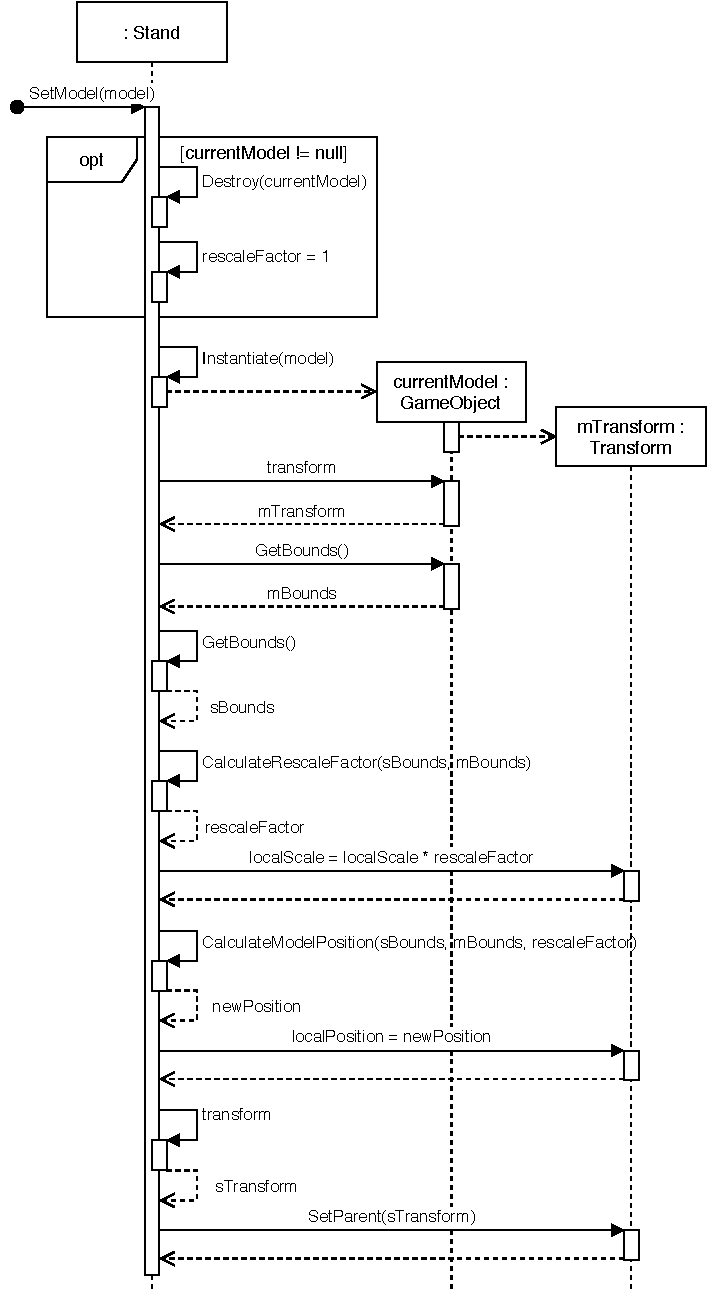
\includegraphics[width=0.8\textwidth]{images/UML-SPlaceModel.pdf}
    \caption{Размещение модели на виртуальном столе.}
    \label{figure:SPlaceModel}
\end{figure}

При размещении новой информационной модели необходимо в первую очередь
произвести ее инспирирование, так как при ее распаковке она не размещается
внутри сцены, а только загружается в память.
Также стоит учесть возможное наличие ранее загруженных моделей.

Для дальнейшего расчета размеров и положения размещаемой модели используются
структуры \emph{Bounds}, представляющие собой параллелепипеды,
ограничивающие область пространства, в которой происходит отрисовка
какого-либо трехмерного объекта. Эти структуры вычисляются как для
размещаемой модели, так и для виртуального стола.
После этого вычисляется вспомогательная величина \emph{rescaleFactor}
согласно формуле:
\[
    r = \frac{
        \min ( sx, sz )
    }{
        \max ( mx, mz )
    }
\]
где $r$ -- \emph{rescaleFactor},
$sx$ и $mx$ -- габариты виртуального стола и информационной модели
вдоль оси $X$, $sz$ и $mz$ -- вдоль оси $Z$.
В дальнейшем \emph{rescaleFactor} используется для вычисления новых
размера и положения модели, а также используется при изменении размеров пользователя.
Формула расчета новых габаритов модели показана на схеме~\ref{figure:SPlaceModel},
а формула для расчета нового положения приведена ниже:

\[
    \vec{p} = \vec{sc} +
    \vec{up} * sy / 2 +
    r * (
        \vec{up} * my / 2 - \vec{mc}
    )
\]
где $\vec{p}$ -- новое положение модели в пространстве (\emph{newPosition}),
$sy$ и $my$ -- габариты виртуального стола и информационной модели
вдоль оси $Y$, а $\vec{sc}$ и $\vec{mc}$ -- их геометрические центры.
В завершение компонент \emph{Transform} размещаемой модели
делается дочерним для \emph{Transform}'а стола.

После размещения модели пользователь может изменять свой размер
за счет вспомогательного компонента \emph{UserScaler},
использующего параметр \emph{rescaleFactor}, рассчитанный
при размещении информационной модели. Изменение размера пользователя
происходит в пределах между естественными размерами пользователя
и размерами пользователя, соответствующими масштабу размещенной модели,
что соответствует алгоритму на схеме~\ref{figure:SSetUserSize}.

\begin{figure}[!htp]
    \centering
    \includegraphics[width=0.6\textwidth]{example-image}
    \caption{Размещение модели на виртуальном столе.}
    \label{figure:SSetUserSize}
    \comment{Scaler.UpdateSize в качестве UserScaler.SetSize}
\end{figure}

\intextcomment{
    Описание UML\dots
}
Пример размещенной на виртуальном столе модели здания отеля
показан на рисунке~\ref{figure:PlacedModelExample}.

\begin{figure}[!htp]
    \centering
    \includegraphics[width=0.6\textwidth]{example-image}
    \caption{Пример размещенной на виртуальном столе
    информационной модели здания.}
    \label{figure:PlacedModelExample}
    \comment{Скриншот}
\end{figure}
